% ------------------------------------------------------------------------
% Projeto de Pesquisa - Estudo de Cálculo
\documentclass[12 pt, openright, twoside, a4paper, english, french, spanish, brazil]{abntex2}

% Pacotes utilizados
\usepackage{lmodern}
\usepackage[utf8]{inputenc}
\usepackage[T1]{fontenc}
\usepackage{indentfirst}
\usepackage{color}
\usepackage{graphicx}
\usepackage{microtype}
\usepackage{amsmath}
\usepackage{amssymb}
\usepackage{pgfplots}
\usepackage{tikz}
\usepackage[brazilian,hyperpageref]{backref}
\usepackage[alf]{abntex2cite}
\usetikzlibrary{arrows.meta,arrows}
\usepackage{bm}

\newcommand\bolden[1]{{\boldmath\bfseries#1}}

% Configurações do pacote backref
\renewcommand{\backrefpagesname}{Citado na(s) página(s):~}
\renewcommand{\backref}{}
\renewcommand*{\backrefalt}[4]{
	\ifcase #1
		Nenhuma citação no texto.
	\or
		Citado na página #2.
	\else
		Citado #1 vezes nas páginas #2.
	\fi}

% Informações para capa e folha de rosto
\titulo{Tópicos de Cálculo Diferencial e Integral}
\autor{Willian Amaral}
\local{Campos do Jordão, SP}
\data{2018}
\instituicao{
	Instituo Federal de São Paulo
	\par
	Campus Campos do Jordão
}
\tipotrabalho{Projeto (Pesquisa)}
\preambulo{Relatório Final de Pesquisa desenvolvido como parte do Projeto de Iniciação Científica, elaborado pelo aluno do curso de Tecnologia em Análise e Desenvolvimento de Sistemas, Willian José do Amaral e orientado pelo Prof. Dr. Sílvio César Otero-Garcia}

% Configurações de aparência (Pegos do Template)
\definecolor{blue}{RGB}{41,5,195}
\makeatletter
\hypersetup{
	pdftitle={\@title}, 
			pdfauthor={\@author},
	    	pdfsubject={\imprimirpreambulo},
		    pdfcreator={LaTeX with abnTeX2},
			pdfkeywords={abnt}{latex}{abntex}{abntex2}{projeto de pesquisa}, 
			colorlinks=true,
	    	linkcolor=blue,
	    	citecolor=blue,
	    	filecolor=magenta,
			urlcolor=blue,
			bookmarksdepth=4
}
\makeatother

\setlength{\parindent}{1.3cm}
\setlength{\parskip}{0.2cm}

% Índice
\makeindex

% Início do documento
\begin{document}

\selectlanguage{brazil}
\frenchspacing

% Capa e folha de rosto
\imprimircapa
\imprimirfolhaderosto

% Início do Trabalho
\textual

% Introdução
\chapter*[Introdução]{Introdução}
\addcontentsline{toc}{chapter}{Introdução}

Este relatório tem como objetivo apresentar os estudos desenvolvidos durante este projeto de pesquisa, bem como explicar as ferramentas utilizadas em referido estudo. O objeto de pesquisa selecionado foi a área matemática de Cálculo - normalmente dividia em duas grandes áreas: o Cálculo Diferencial e o Cálculo Integral - e sua relação com a área de Desenvolvimento de Sistemas. Para isso, foram utilizadas ferramentas usadas principalmente no campo da Computação e Engenharia de Software, como a linguagem de scripts e formatação de textos \LaTeX, o editor de textos de código-fonte Sublime Text, e os respectivos pacotes adicionais à essas ferramentas na edição e documentação de textos científicos e matemáticos. Para isso, a metodologia de pesquisa utilizada foi a leitura, resolução e formatação de exercícios selecionados do livro Cálculo A - Funções, Limites, Derivação e Integração, de Diva Marília Flemming e Mirian Buss Gonçalves.

% Capítulo 1 - Sobre Cálculo
\chapter{Sobre Cálculo}
\index{sobre calculo}

A fim de contextualizar o desenvolvimento do projeto de pesquisa, é importante apresentarmos uma breve análise do estudo de Cálculo. Por isso, pontuamos questões relevantes ao histório desta área de estudo. \\
A criação do Cálculo contou com uma variedade de pesquisadores e teóricos matemáticos, que buscavam solucionar problemas matemáticos com alto nívro de dificuldade, como a ideia de infinito, presente no estudo do movimento e as razões entre grandezas de segmentos.

Embora inicialmente não houvessem sistematizações ou lógicas estruturadas para a resolução destes problemas, foi o estudo conjunto de matemáticos ao longo da história que deu origem aos principais pilares do Cálculo: a Derivada e a Integral. 

É possível traçar o desenvolvimento da área de Cálculo em diversos períodos da história, notavelmente nas eras antiga, medieval e moderna. O Cálculo Integral foi introduzido na era antiga, baseado no cálculo de volumes e áreas, como o papiro égípcio de Moscow datado do ano 1800 a.C., que mostra como os egípcios trabalhavam com o volume de um \textit{``frustum''} piramidal.

As ideias dos matemáticos egípcios foram levadas adiante, gerando a criação da heurística, que se aproxima do Cálculo Integral. Os mesmos métodos foram redescobertos na China no século III d.C por Liu Hui, que o utilizou para encontrar a área do Círculo. 
Séculos depois, em XII d.C. o matemático persa Sharaf al-Din al-tusi descobriu a derivada de polimônios cúbicos, o que levaria a um importante passo para a criação da área de estudo do Cálculo Diferencial. Essa área também está intrínsecamente ligada ao desenvolvimento do estudo das tangentes, que acontecia desde a época dos gregos antigos, e também se tornou parte da Geometria Analítica. 
%%CONTINUAR

% Capítulo 2 - Ferramentas Computacionais
\chapter{Ferramentas Computacionais}
\index{ferramentas computacionais}

A fim de salientar a importância desse estudo para a área de Sistemas da Informação e Computação, foram utilizadas diversas ferramentas computacionais durante o desenvolvimento do projeto de Iniciação Científica. Entre elas, o estudo da linguagem de formatação tipográfica \LaTeX.

% Capítulo 3 - Resolução dos Exercícios
\chapter{Resolução dos Exercícios}
\index{resolucao exercicios}

Esse capítulo contém a resolução de exercícios selecionados da bibliografia, afim de facilitar e melhorar o entendimento dos assuntos tratados.

%% Números Reais
\section{Números Reais}

O estudo de números reais engloba os conjuntos dos números naturais, inteiros, racionais e irracionais. Os exercícios a seguir demonstram algumas operações e cálculos envolvendo o conjunto. 

\subsection{Exercícios}
1. Determinar todos os intervalos de números que satisfaçam as desigualdades abaixo. Fazer a representação gráfica.

\textit{(a)} $3 - x < 5 + 3x$

Resolução:

\begin{align*}
\begin{split}
3x + x &< -5 -3 \\
4x &< -2 \\
x &< -\frac{2}{4} \\
x &< -\frac{1}{2}
\end{split}
\end{align*}
\bigskip

Resposta: \bolden{$(-\frac{1}{2},+\infty)$}

Representação Gráfica:

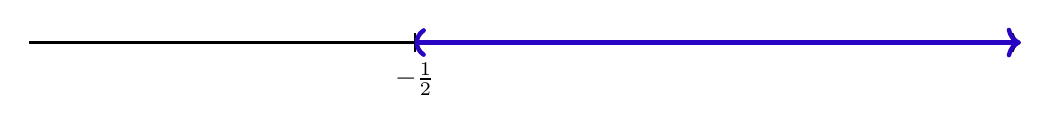
\begin{tikzpicture}[scale=7]
\draw[->, thick] (-0.1,0) -- (1.7,0);
\foreach \x/\xtext in {0.6/$-\frac{1}{2}$}
    \draw[thick] (\x,0.5pt) -- (\x,-0.5pt) node[below] {\xtext};
\draw[{(->}, ultra thick, blue] (0.6,0) -- (1.7,0);
\end{tikzpicture}


\textit{(b)} $2 > - 3 - 3x \geq -7$

Resolução:

\begin{align*}
\begin{split}
3 + 2 &> -3x \geq -7 + 3 \\
5 &> -3x \geq -4 \\
-\frac{5}{3} &< x \leq \frac{4}{3}
\end{split}
\end{align*}

Resposta: \bolden{$(-\frac{5}{3},\frac{4}{3}]$}

Representação Gráfica:

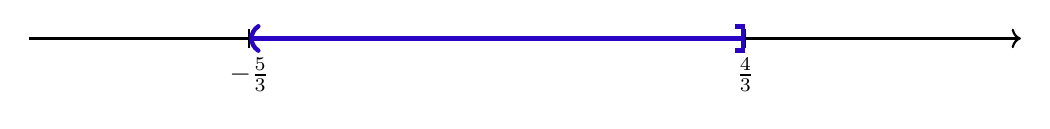
\begin{tikzpicture}[scale=7]
\draw[->, thick] (-0.1,0) -- (1.7,0);
\foreach \x/\xtext in {0.3/$-\frac{5}{3}$,1.2/$\frac{4}{3}$}
    \draw[thick] (\x,0.5pt) -- (\x,-0.5pt) node[below] {\xtext};
\draw[{(-]}, ultra thick, blue] (0.3,0) -- (1.2,0);
\end{tikzpicture}
\bigskip


\textit{(c)} $x^2 \leq 9$

Resolução:

\begin{align*}
\begin{split}
x &\leq \sqrt{9} \\
x(1) &\leq 3  \\
x(2) &\geq -3 
\end{split}
\end{align*}

Resposta: \bolden{$[-3,3]$}

Representação Gráfica:

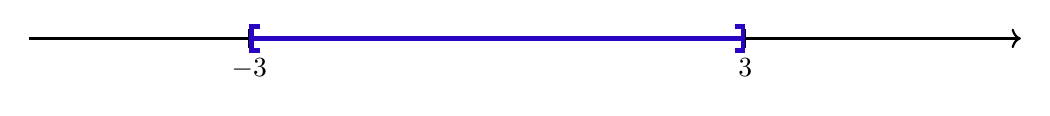
\begin{tikzpicture}[scale=7]
\draw[->, thick] (-0.1,0) -- (1.7,0);
\foreach \x/\xtext in {0.3/$-3$,1.2/$3$}
    \draw[thick] (\x,0.5pt) -- (\x,-0.5pt) node[below] {\xtext};
\draw[{[-]}, ultra thick, blue] (0.3,0) -- (1.2,0);
\end{tikzpicture}

\bigskip


\textit{(d)} $1 - x - 2x^2 \geq 0$

Resolução:

\begin{align*}
\begin{split}
x &\geq \frac{-(-1) \pm \sqrt{1 -4(-2)1}}{2(-2)} \\
x &\geq \frac{1 \pm \sqrt{9}}{-4} \\
x &\geq \frac{1 \pm 3}{-4} \\
(1) x &\geq \frac{4}{-4} \\
(1) x &\geq -1 \\
(2) x &\geq \frac{-2}{-4} \\
(2) x &\leq \frac{1}{2} \\
\end{split}
\end{align*}

Resposta: \bolden{$[-1,\frac{1}{2}]$}

Representação Gráfica:

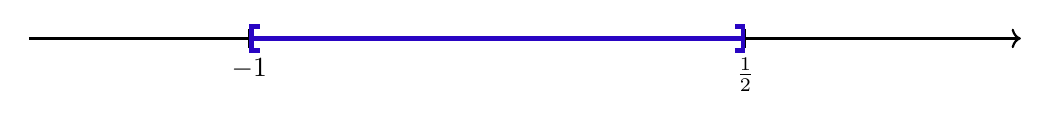
\begin{tikzpicture}[scale=7]
\draw[->, thick] (-0.1,0) -- (1.7,0);
\foreach \x/\xtext in {0.3/$-1$,1.2/$\frac{1}{2}$}
    \draw[thick] (\x,0.5pt) -- (\x,-0.5pt) node[below] {\xtext};
\draw[{[-]}, ultra thick, blue] (0.3,0) -- (1.2,0);
\end{tikzpicture}


\textit{(e)} $x^3 + 1 > x^2 + x$

Resposta: \bolden{$(-1,1) \cup (1,+\infty)$}

Representação Gráfica:

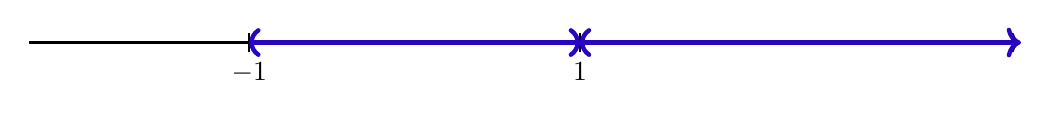
\begin{tikzpicture}[scale=7]
\draw[->, thick] (-0.1,0) -- (1.7,0);
\foreach \x/\xtext in {0.3/$-1$,0.9/$1$}
    \draw[thick] (\x,0.5pt) -- (\x,-0.5pt) node[below] {\xtext};
\draw[{(-)}, ultra thick, blue] (0.3,0) -- (0.9,0);
\draw[{(->}, ultra thick, blue] (0.9,0) -- (1.7,0);
\end{tikzpicture}

\bigskip
\bigskip


\textit{(f)} $\displaystyle \frac{2}{x - 2} \leq \frac{x + 2}{x - 2} \leq 1$

\bigskip

Resposta: \bolden{$(-\infty,0]$}

Representação Gráfica:

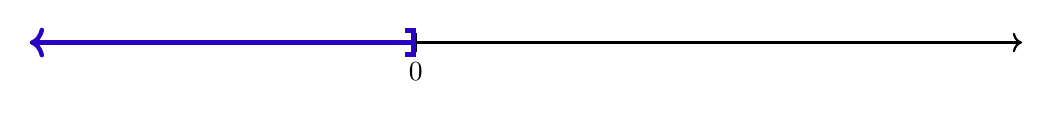
\begin{tikzpicture}[scale=7]
\draw[->, thick] (-0.1,0) -- (1.7,0);
\foreach \x/\xtext in {0.6/$0$}
    \draw[thick] (\x,0.5pt) -- (\x,-0.5pt) node[below] {\xtext};
\draw[{<-]}, ultra thick, blue] (-0.1,0) -- (0.6,0);
\end{tikzpicture}

\bigskip
\bigskip


\textit{(g)} $\displaystyle \frac{x}{x - 3} < 4$

\bigskip

Resposta: \bolden{$(-\infty,3) \cup (4,+\infty)$}

Representação Gráfica:

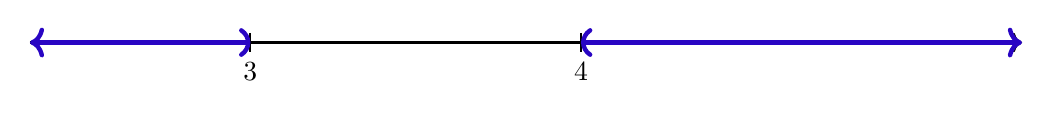
\begin{tikzpicture}[scale=7]
\draw[->, thick] (-0.1,0) -- (1.7,0);
\foreach \x/\xtext in {0.3/$3$,0.9/$4$}
    \draw[thick] (\x,0.5pt) -- (\x,-0.5pt) node[below] {\xtext};
\draw[{<-)}, ultra thick, blue] (-0.1,0) -- (0.3,0);
\draw[{(->}, ultra thick, blue] (0.9,0) -- (1.7,0);
\end{tikzpicture}

\bigskip
\bigskip


\textit{(h)} $\displaystyle \frac{3}{x - 5} \leq 2$

\bigskip

Resposta: \bolden{$(-\infty,5) \cup [\frac{13}{2},+\infty)$}

Representação Gráfica:

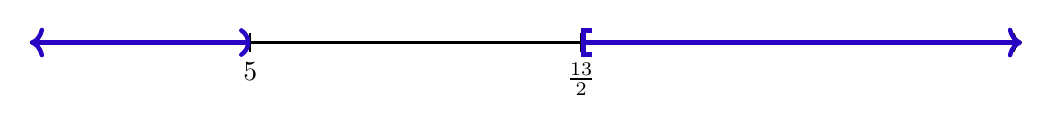
\begin{tikzpicture}[scale=7]
\draw[->, thick] (-0.1,0) -- (1.7,0);
\foreach \x/\xtext in {0.3/$5$,0.9/$\frac{13}{2}$}
    \draw[thick] (\x,0.5pt) -- (\x,-0.5pt) node[below] {\xtext};
\draw[{<-)}, ultra thick, blue] (-0.1,0) -- (0.3,0);
\draw[{[->}, ultra thick, blue] (0.9,0) -- (1.7,0);
\end{tikzpicture}

\bigskip


\textit{(i)} $x^3 - 3x + 2 \leq 0$

Resposta: \bolden{$(-\infty,-2] \cup {1})$}

Representação Gráfica:

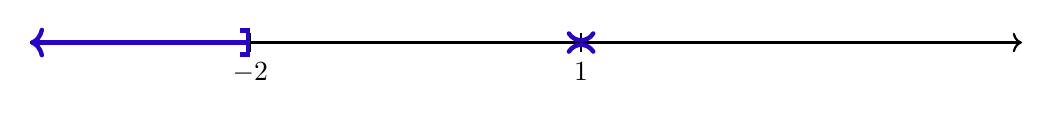
\begin{tikzpicture}[scale=7]
\draw[->, thick] (-0.1,0) -- (1.7,0);
\foreach \x/\xtext in {0.3/$-2$,0.9/${1}$}
    \draw[thick] (\x,0.5pt) -- (\x,-0.5pt) node[below] {\xtext};
\draw[{<-]}, ultra thick, blue] (-0.1,0) -- (0.3,0);
\draw[{(-)}, ultra thick, blue] (0.9,0) -- (0.9,0);
\end{tikzpicture}

\bigskip


\textit{(j)} $8x^3 - 4x^2 - 2x + 1 < 0$

Resposta: \bolden{$(-\infty,-\frac{1}{2})$}

Representação Gráfica:

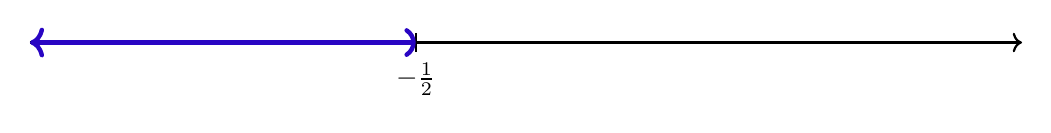
\begin{tikzpicture}[scale=7]
\draw[->, thick] (-0.1,0) -- (1.7,0);
\foreach \x/\xtext in {0.6/$-\frac{1}{2}$}
    \draw[thick] (\x,0.5pt) -- (\x,-0.5pt) node[below] {\xtext};
\draw[{<-)}, ultra thick, blue] (-0.1,0) -- (0.6,0);
\end{tikzpicture}
\bigskip


2. Resolver as equações em I\!R.

\textit{(a)} $|5x - 3| = 12$

Resolução:

\begin{align*}
\begin{split}
|5x -3| &= 12 \\
5x &= 12 + 3 \\
x &= \frac{15}{5} \\
x &= 3 \\
\end{split}
\end{align*}
\begin{center}
ou
\end{center}
\begin{align*}
\begin{split}
|5x - 3| &= -12 \\
5x &= -12 + 3 \\
5x &= -9 \\
x &= -\frac{9}{5}
\end{split}
\end{align*}

Resposta: \bolden{$|x| = 3$ ou $-\frac{9}{5}$}


\bigskip


\textit{(b)} $|2x - 3| = |7x - 5|$

Resolução:

\begin{align*}
\begin{split}
|2x -3| &= |7x -5| \\
2x - 7x &= -5 + 3 \\
-5x &= -2 \\
x &= \frac{-2}{-5} \\
x &= \frac{2}{5}
\end{split}
\end{align*}
\begin{center}
ou
\end{center}
\begin{align*}
\begin{split}
|2x -3| &= |7x -5| \\
2x &= -7x + 5 + 3 \\
9x &= 8 \\
x &= \frac{8}{9}
\end{split}
\end{align*}

Resposta: \bolden{$|x| = \frac{2}{5}$ ou $\frac{8}{9}$}


\bigskip


\textit{(c)} $\displaystyle \left|\frac{3x + 8}{2x - 3}\right| = 4$

\bigskip

Resolução:

\begin{align*}
\begin{split}
3x + 8 &= 4(2x - 3) \\
3x &= 8x - 12 - 8 \\
-5x &= -20 \\
x &= \frac{-20}{-5} \\
|x| &= 4
\end{split}
\end{align*}
\begin{center}
ou
\end{center}
\begin{align*}
\begin{split}
3x + 8 &= -4(2x - 3) \\
3x &= -8x + 12 - 8 \\
11x &= 4 \\
|x| &= \frac{4}{11}
\end{split}
\end{align*}

Resposta: \bolden{$|x| = 4$ ou $\frac{4}{11}$}


\bigskip


\textit{(d)} $|9x| - 11 = x$

Resolução: 

\begin{align*}
\begin{split}
|9x| &= x + 11 \\
9x - x &= 11 \\
x &= \frac{11}{8} 
\end{split}
\end{align*}
\begin{center}
ou
\end{center}
\begin{align*}
\begin{split}
|9x| &= -(x + 11) \\
9x + x &= -11 \\
x &= -\frac{11}{10} 
\end{split}
\end{align*}

Resposta: \bolden{$|x| = \frac{11}{8}$ ou $\frac{11}{10}$}


\bigskip


%% Funções
\section{Funções}

O conceito de função refere-se essencialmente à correspondência entre conjuntos. Uma função associa elementos de um conjunto a elementos de outro conjunto. Recursos computacionais são ainda mais importantes no estudo de funções, uma vez que auxiliam na visualização das propriedades e características das funções. 

\subsection{Exercícios}

1. Usando uma ferramenta gráfica, traçar as curvas definidas pelas equações dadas, identificando as que representam o gráfico de uma função $y = f(x)$. Neste caso, determine a função, o domínio e o conjunto imagem. 

\textit{(a)} $y = 3x - 1$

Resolução:

\begin{tikzpicture}
\begin{axis}[
    axis lines = middle,
    xlabel = $x$,
    ylabel = {$f(x)$},
]
\addplot [
    domain=-10:10, 
    samples=100, 
    color=blue,
    ]
    {3*x - 1};
\end{axis}
\end{tikzpicture}

Resposta: É uma função

$f(x) = 3x - 1$ 

$D(f) = \mathbb{R}$

$Im(f) = \mathbb{R}$
\bigskip

\textit{(b)} $y - x^2 = 0$

Resolução:

\begin{tikzpicture}
\begin{axis}[
    axis lines = middle,
    xlabel = $x$,
    ylabel = {$f(x)$},
]
\addplot [
    domain=-10:10, 
    samples=100, 
    color=blue,
    ]
    {x^2};
\end{axis}
\end{tikzpicture}

Resposta: É uma função

$f(x) = x^2$ 

$D(f) = \mathbb{R}$

$Im(f) = \mathbb{R}\star$
\bigskip

\textit{(c)} $y^2 - x = 0$

Resolução:

\begin{tikzpicture}
\begin{axis}[
    axis lines = middle,
    xlabel = $x$,
    ylabel = {$f(x)$},
]
\addplot [
    domain=-10:10, 
    samples=100, 
    color=blue,
    ]
    {sqrt(x)};
\addplot [
    domain=-10:10, 
    samples=100, 
    color=blue,
    ]
    {-sqrt(x)};
\end{axis}
\end{tikzpicture}

Resposta: Não é uma função
\bigskip

\textit{(d)} $y + \sqrt{4 - x^2} = 0$

Resolução:

\begin{tikzpicture}
\begin{axis}[
    axis lines = middle,
    xlabel = $x$,
    ylabel = {$f(x)$},
]
\addplot [
    domain=-10:10, 
    samples=100, 
    color=blue,
    ]
    {-sqrt(4 - x^2)};
\end{axis}
\end{tikzpicture}

Resposta: É uma função

$f(x) = -\sqrt{4 - x^2}$ 

$D(f) = [-2,2]$

$Im(f) = [-2,0]$
\bigskip

\textit{(e)} $x^2 + y^2 = 16$

Resolução:

\begin{tikzpicture}
\begin{axis}[
    axis lines = middle,
    xlabel = $x$,
    ylabel = {$f(x)$},
]
\addplot [
    domain=-10:10, 
    samples=100, 
    color=blue,
    ]
    {sqrt(16 - x^2)};
\addplot [
    domain=-10:10, 
    samples=100, 
    color=blue,
    ]
    {-sqrt(16 - x^2)};
\end{axis}
\end{tikzpicture}

Resposta: Não é uma função
\bigskip

\textit{(f)} $y = \frac{1}{x}$

Resolução:

\begin{tikzpicture}
\begin{axis}[
    axis lines = middle,
    xlabel = $x$,
    ylabel = {$f(x)$},
]
\addplot [
    domain=-10:10, 
    samples=100, 
    color=blue,
    ]
    {1/x};
\end{axis}
\end{tikzpicture}

Resposta: É uma função

$f(x) = \frac{1}{x}$ 

$D(f) = \mathbb{R} - \{0\}$

$Im(f) = \mathbb{R} - \{0\}$
\bigskip

\textit{(g)} $y - x^2 = 11$

Resolução:

\begin{tikzpicture}
\begin{axis}[
    axis lines = middle,
    xlabel = $x$,
    ylabel = {$f(x)$},
]
\addplot [
    domain=-10:10, 
    samples=100, 
    color=blue,
    ]
    {11 + x^2};
\end{axis}
\end{tikzpicture}

Resposta: É uma função

$f(x) = 11 + x^2$ 

$D(f) = \mathbb{R}$

$Im(f) = [11,+\infty)$
\bigskip

\end{document}